% Digital Logic Lab 10 7-Segment Display with Time-Division Multiplexing
% Created: 2020-04-16, Megan Gordon

%==========================================================
%=========== Document Setup  ==============================

% Formatting defined by class file
\documentclass[11pt]{article}

% ---- Document formatting ----
\usepackage[margin=1in]{geometry}	% Narrower margins
\usepackage{booktabs}				% Nice formatting of tables
\usepackage{graphicx}				% Ability to include graphics

%\setlength\parindent{0pt}	% Do not indent first line of paragraphs 
\usepackage[parfill]{parskip}		% Line space b/w paragraphs
%	parfill option prevents last line of pgrph from being fully justified

% Parskip package adds too much space around titles, fix with this
\RequirePackage{titlesec}
\titlespacing\section{0pt}{8pt plus 4pt minus 2pt}{3pt plus 2pt minus 2pt}
\titlespacing\subsection{0pt}{4pt plus 4pt minus 2pt}{-2pt plus 2pt minus 2pt}
\titlespacing\subsubsection{0pt}{2pt plus 4pt minus 2pt}{-6pt plus 2pt minus 2pt}

% ---- Hyperlinks ----
\usepackage[colorlinks=true,urlcolor=blue]{hyperref}	% For URL's. Automatically links internal references.

% ---- Code listings ----
\usepackage{listings} 					% Nice code layout and inclusion
\usepackage[usenames,dvipsnames]{xcolor}	% Colors (needs to be defined before using colors)

% Define custom colors for listings
\definecolor{listinggray}{gray}{0.98}		% Listings background color
\definecolor{rulegray}{gray}{0.7}			% Listings rule/frame color

% Style for Verilog
\lstdefinestyle{Verilog}{
	language=Verilog,					% Verilog
	backgroundcolor=\color{listinggray},	% light gray background
	rulecolor=\color{blue}, 			% blue frame lines
	frame=tb,							% lines above & below
	linewidth=\columnwidth, 			% set line width
	basicstyle=\small\ttfamily,	% basic font style that is used for the code	
	breaklines=true, 					% allow breaking across columns/pages
	tabsize=3,							% set tab size
	commentstyle=\color{gray},	% comments in italic 
	stringstyle=\upshape,				% strings are printed in normal font
	showspaces=false,					% don't underscore spaces
}

% How to use: \Verilog[listing_options]{file}
\newcommand{\Verilog}[2][]{%
	\lstinputlisting[style=Verilog,#1]{#2}
}




%======================================================
%=========== Body  ====================================
\begin{document}

\title{ELC 2137 Lab 10: 7-Segment Display with Time-Division Multiplexing}
\author{Megan Gordon}

\maketitle


\section*{Summary}

This lab looks to expand on previous labs by expanding into larger systems with more modules. It allowed us to learn how to create a 7-segment multiplexer utilizing counters. In completing this lab, the following skills were gained: ability to recognize synchronous design methodology for regular sequential circuits, the ability to develop a parameterized counter-timer module, the ability to implement a clock-driven, 4-digit display using multiple instances of a counter module. 



\section*{Results}

\textbf{Deliverable Questions:}

\medskip
\textbf{a)} The three main groups of the RTL definition of sequential logic are the set of registers in the system, the operations performed on the data stored in the registers, and the control that supervises the sequence of operations in the system.

\textbf{b)} Here is an annotated figure to distinguish components in this example our register is a counter:
\begin{figure}[ht]\centering
	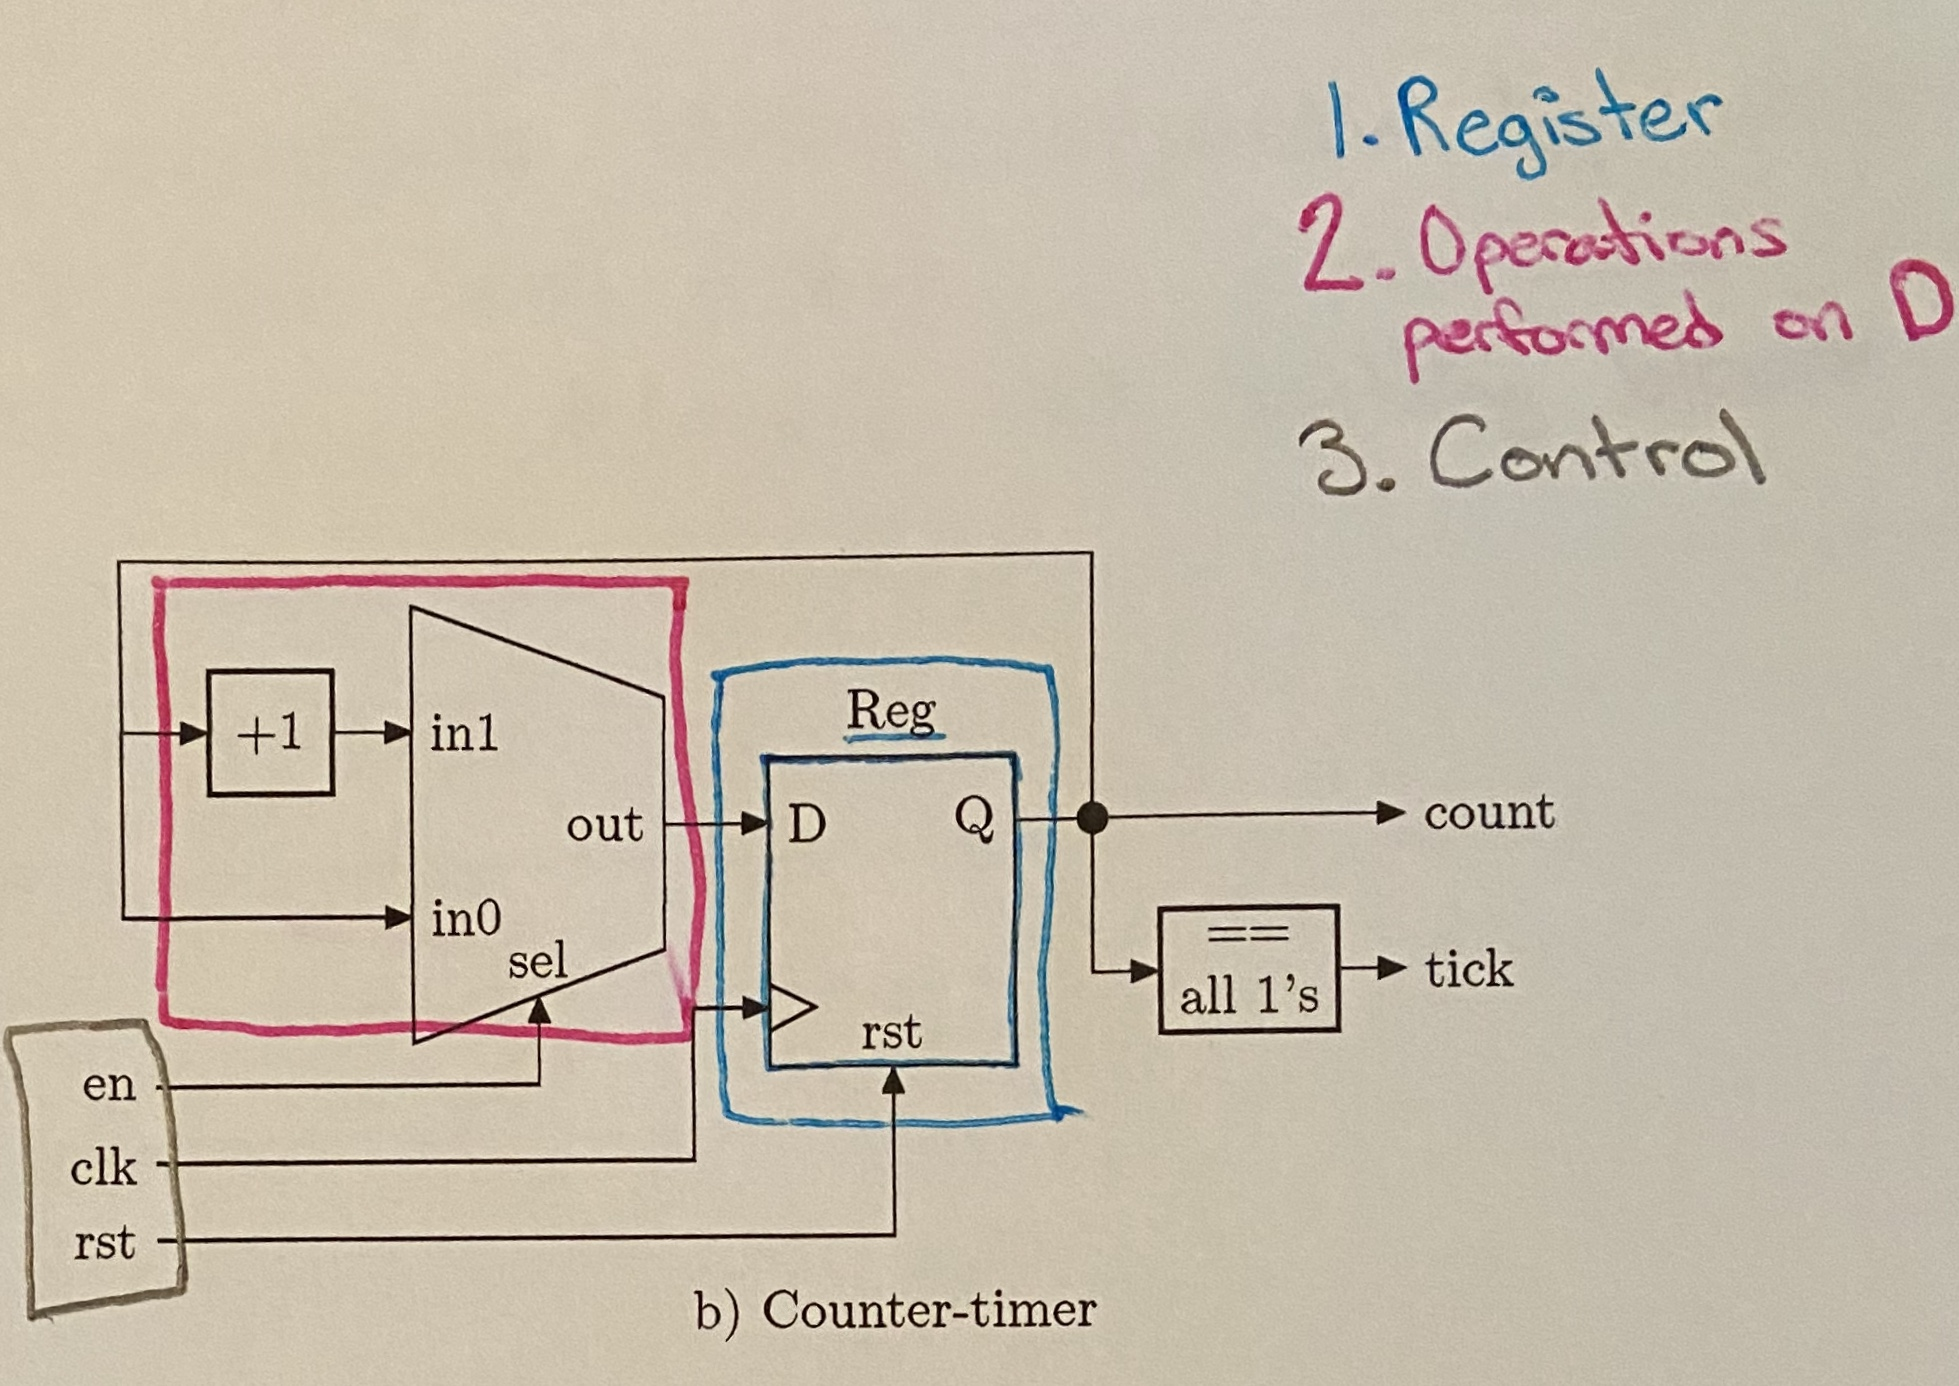
\includegraphics[angle=0, width=0.5\textwidth]{IMG_6712.jpg}
\end{figure}

\textbf{c)} Using a shift register (low to high) instead of a counter would result in line $Q-next<=(LSB-in, Q-next[N-2:0])$

\clearpage

\textbf{Below are the simulations with ERTs for 2 modules (counter and a 7-seg driver) and pictures of the board for each step in the operation list for on-board testing.} 
\bigskip
\bigskip
\bigskip

\begin{figure}[ht]\centering
	\begin{tabular}{l|rrrrrrrrrrr}
		Time (ns): & 0-5 & 5-10 & 10-15 & 15-20 & 20-25 & 25-30 & 30-35 & 35-40 & 40-45 & 45-50 & 50-55 \\
		\midrule 
		clk & 0 & 1 & 0 & 1 & 0 & 1 & 0 & 1 & 0 & 1 & 0 \\
		en & 0 & 0 & 1 & 0 & 1 & 0 & 1 & 0 & 1 & 0 & 1 \\
		rst & 0 & 1 & 0 & 0 & 0 & 0 & 0 & 0 & 0 & 0 & 0 \\
		\midrule
		count & X & 0 & 0 & 1 & 1 & 2 & 2 & 3 & 3 & 4 & 4  \\
		clkA & X & 0 & 0 & 1 & 1 & 0 & 0 & 1 & 1 & 0 & 0  \\
		clkB & X & 0 & 0 & 0 & 0 & 1 & 1 & 1 & 1 & 0 & 0  \\
		clkC & X & 0 & 0 & 0 & 0 & 0 & 0 & 0 & 0 & 1 & 1  \\
		\bottomrule
	\end{tabular}\medskip

	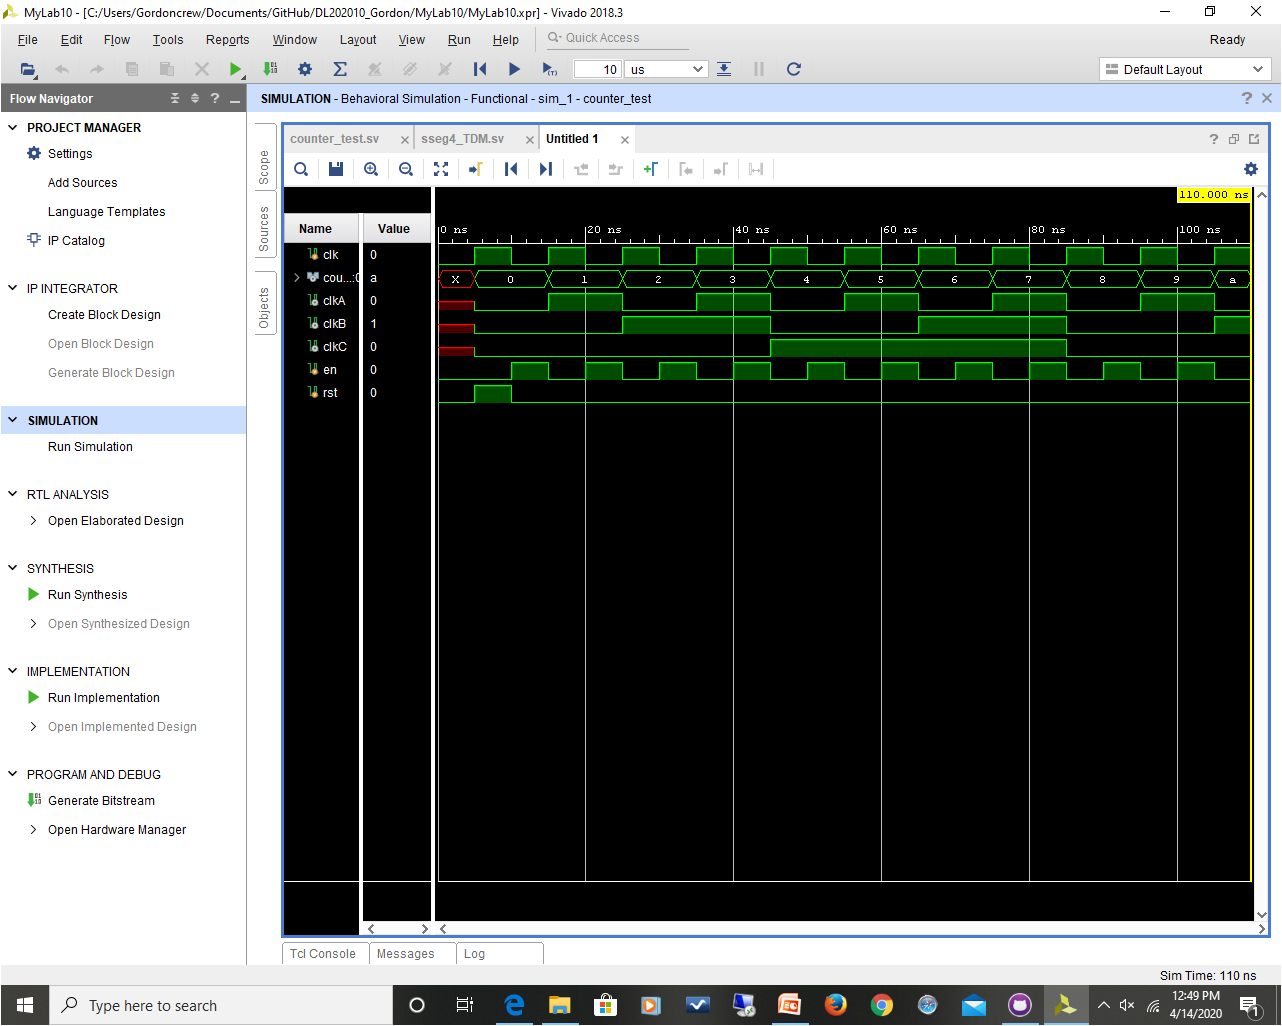
\includegraphics[width=1.15\textwidth, trim=7.5cm 14cm 0cm 4cm,clip]{counter.png}
	\caption{Counter ERT and Testbench Results}
	\label{fig:sim_with_table}
\end{figure}


\begin{figure}[ht]\centering
	\begin{tabular}{l|rrrrrrrrrrrr}
		Time (ms): & 0-5 & 5-10 & 10-15 & 15-20 & 20-25 & 25-30 & 30-35 & 35-40 & 40-45 & 45-50 & 50-55 & 55-60  \\
		\midrule 
		hexdec & 0 & 0 & 0 & 0 & 0 & 1 & 1 & 1 & 1 & 1 & 1 & 1  \\
		sign & 0 & 0 & 0 & 0 & 0 & 0 & 0 & 0 & 0 & 0 & 1 & 1  \\
		rst & 0 & 1 & 0 & 0 & 0 & 0 & 0 & 0 & 0 & 0 & 0 & 1  \\
		\midrule
		an[3] & 1 & 1 & 1 & 1-0 & 0-1 & 1 & 1 & 1-0 & 0-1 & 1 & 1 & 1-0 \\
		an[2] & 1 & 1 & 1-0 & 0-1 & 1 & 1 & 1-0 & 0-1 & 1 & 1 & 1-0 & 0-1\\
		an[1] & 1 & 1-0 & 0-1 & 1 & 1 & 1-0 & 0-1 & 1 & 1 & 1-0 & 0-1 & 1\\
		an[0] & 0 & 0-1 & 1 & 1 & 1-0 & 0-1 & 1 & 1 & 1-0 & 0-1 & 1 & 1  \\
		seg (hex) & 30 & 78 & 02 & 79 & 30 & 12 & 02 & 79 & 79 & 12 & 02 & 3E \\
		\bottomrule
	\end{tabular}\medskip
	
	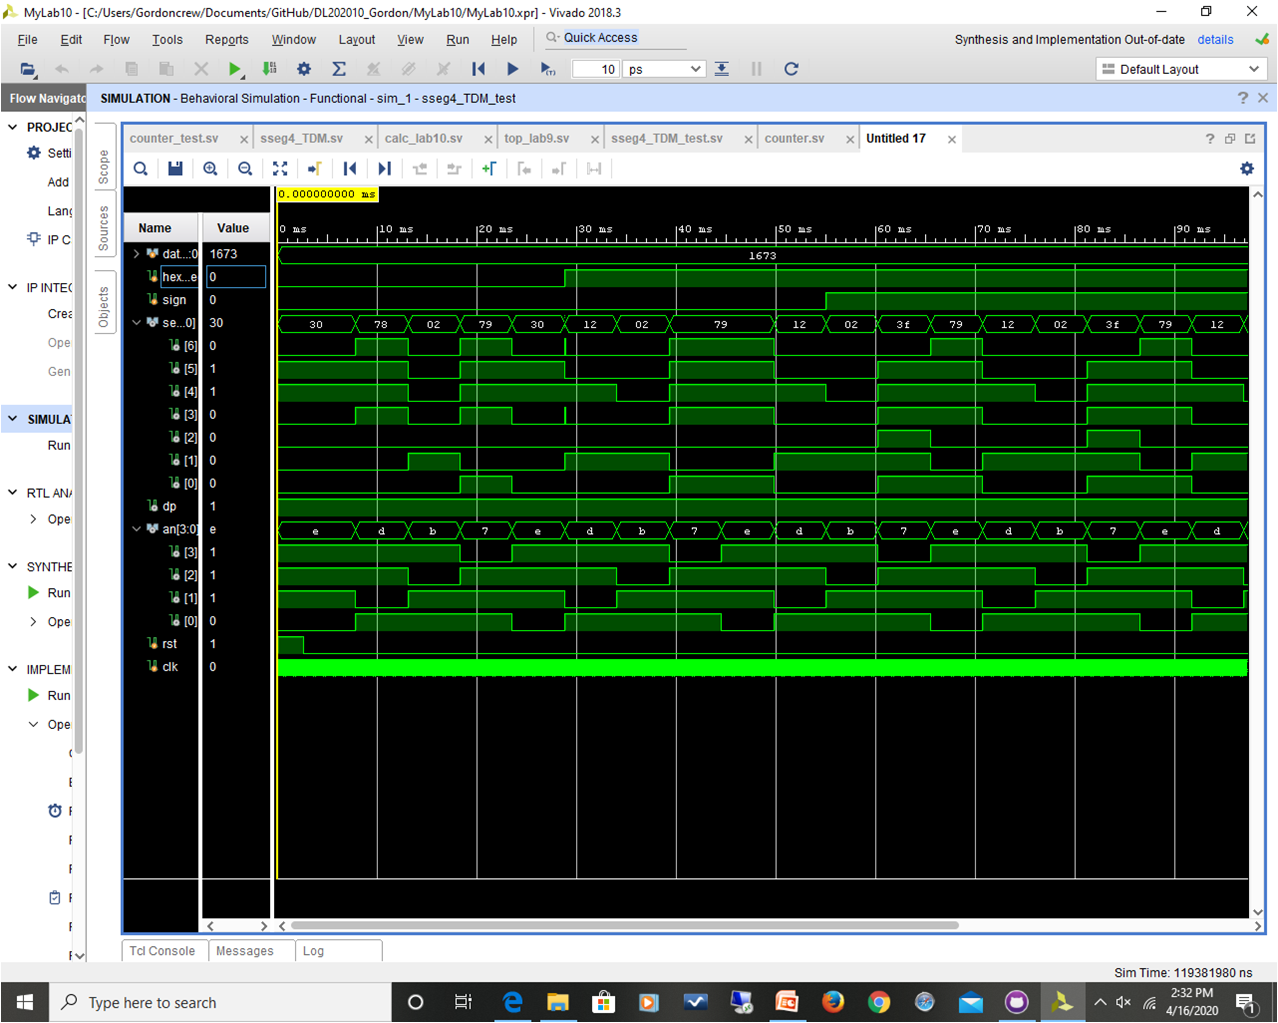
\includegraphics[width=1.15\textwidth, trim=2cm 5.5cm 2cm 4.0cm,clip]{ssegtest.png}
	\caption{7-Seg Driver ERT when data is 1673 and Testbench Results}
	\label{fig:sim_with_table}
\end{figure}


\clearpage

\begin{figure}[ht]\centering
	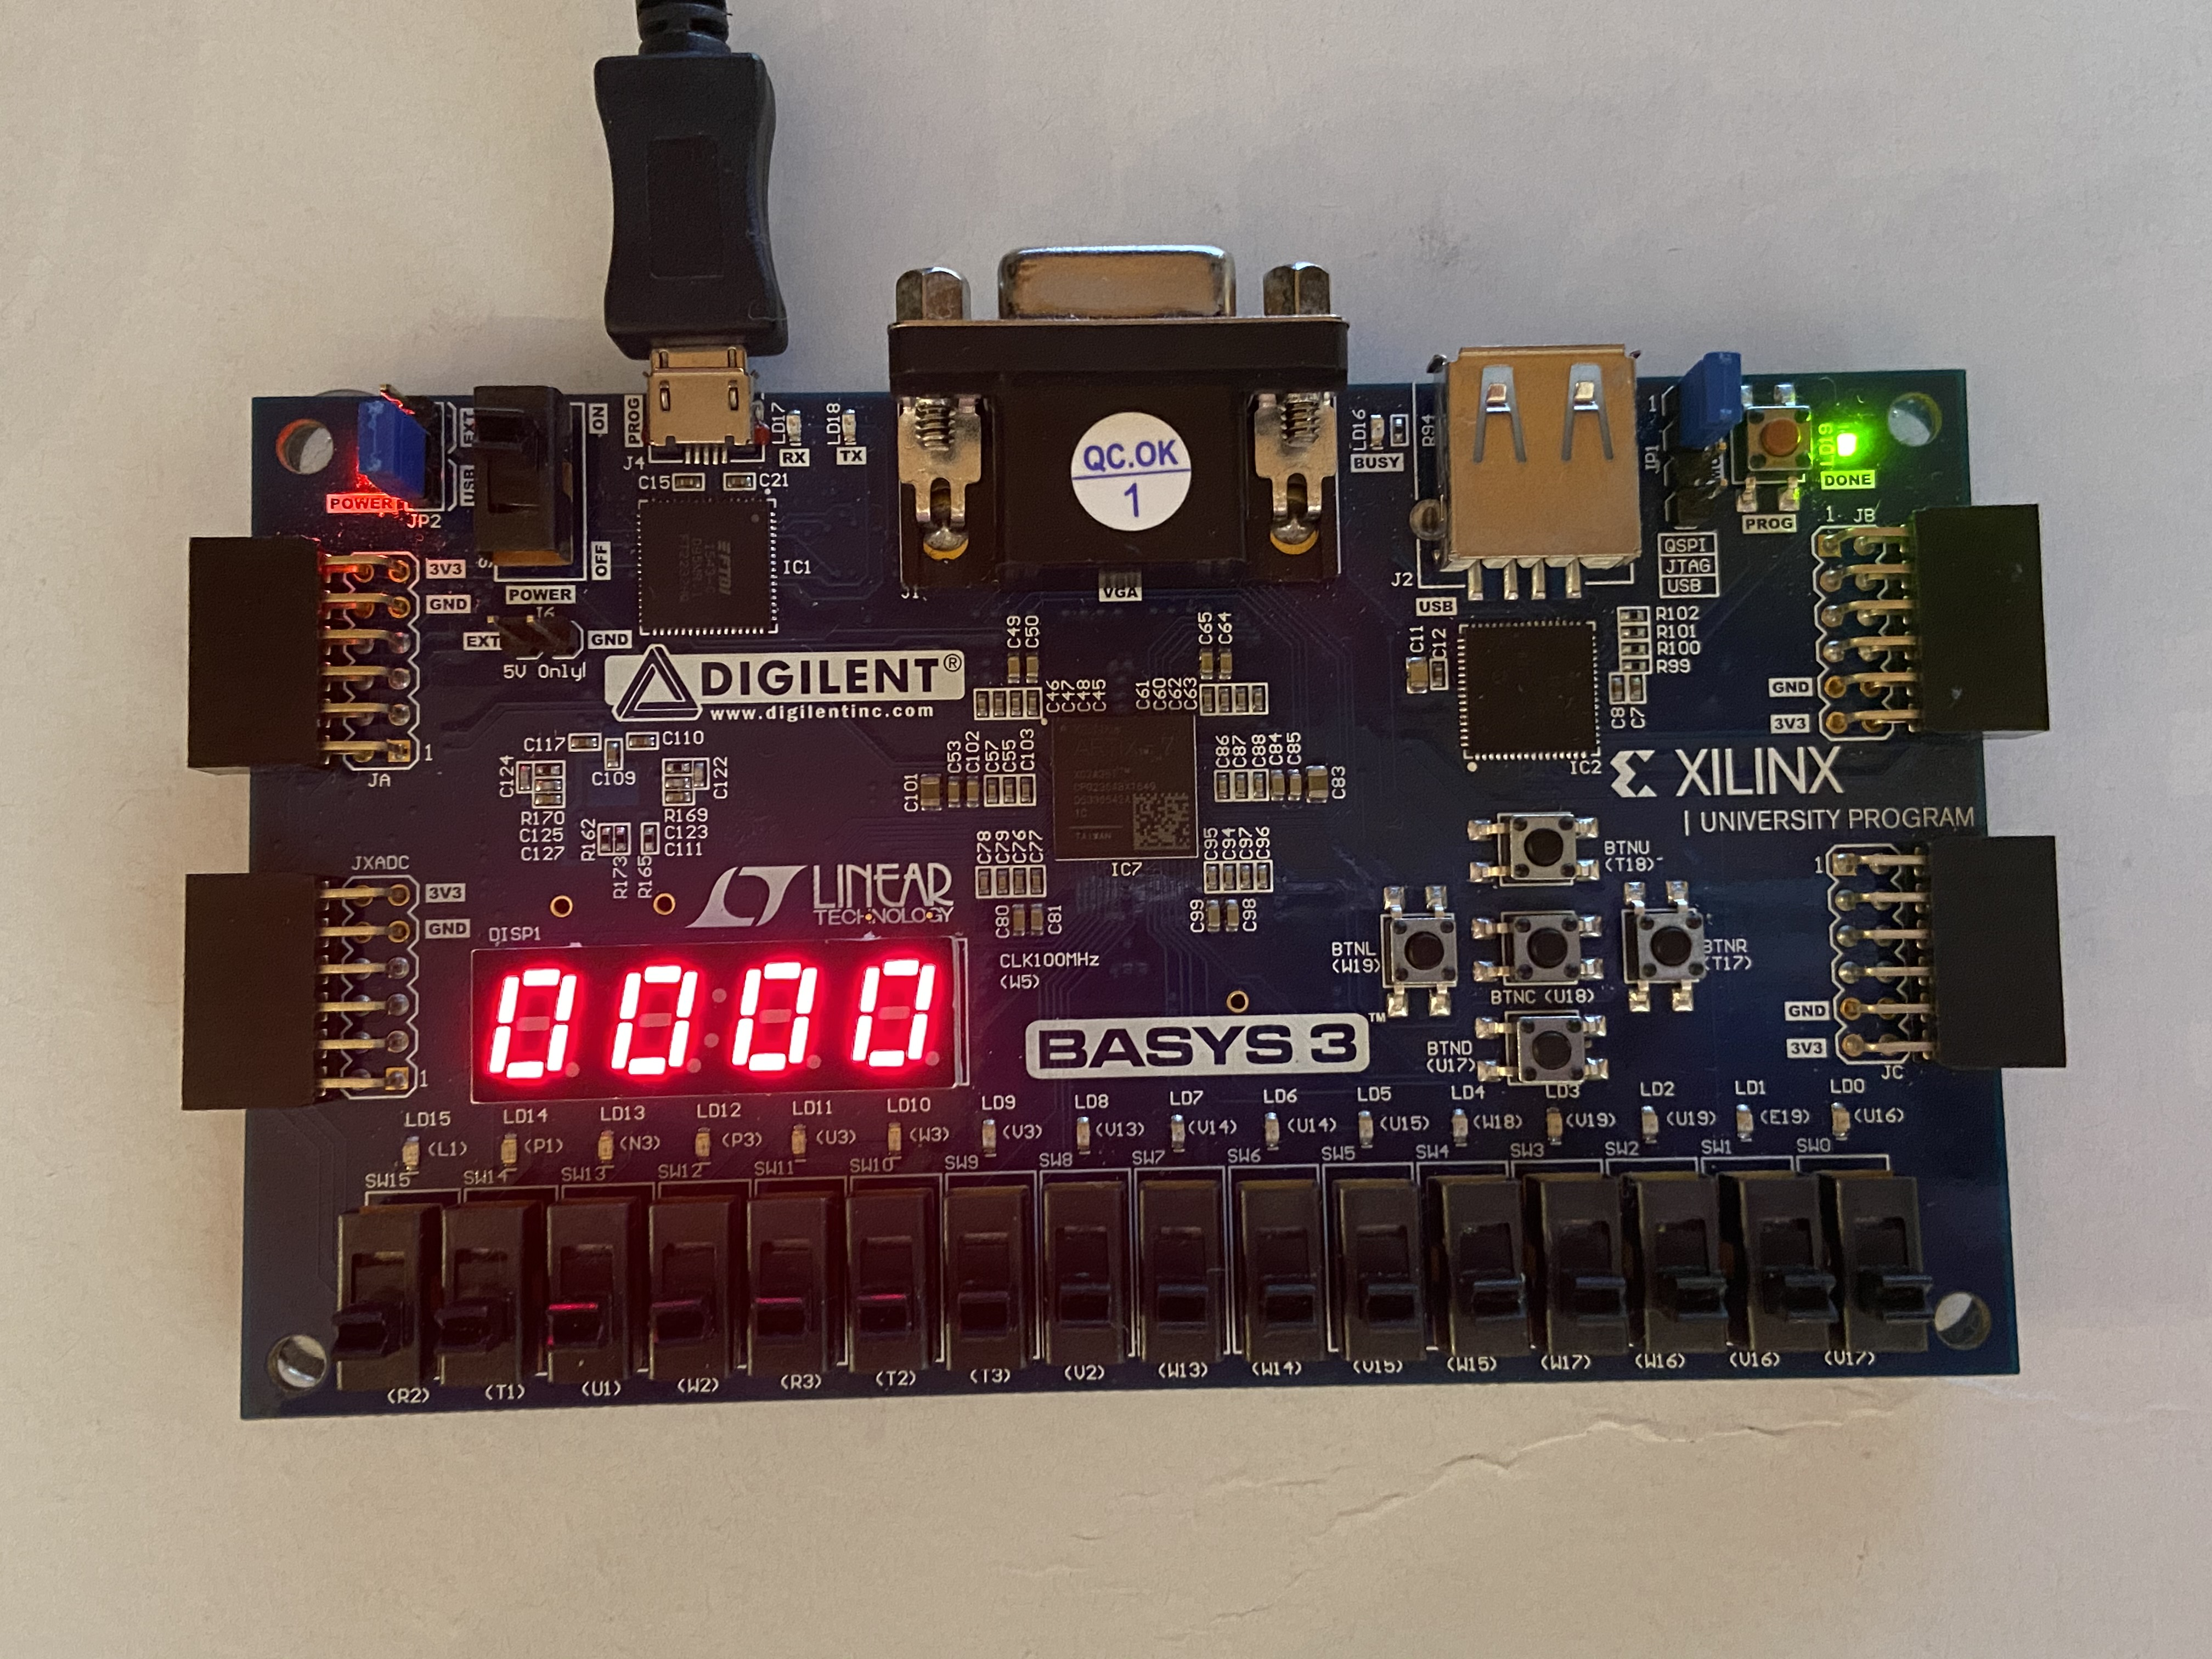
\includegraphics[angle=0, width=1.0\textwidth]{IMG_6746.jpg}
	\caption{Testing Step 1}
	\label{fig:sim_with_table}
\end{figure}
\clearpage

\begin{figure}[ht]\centering
	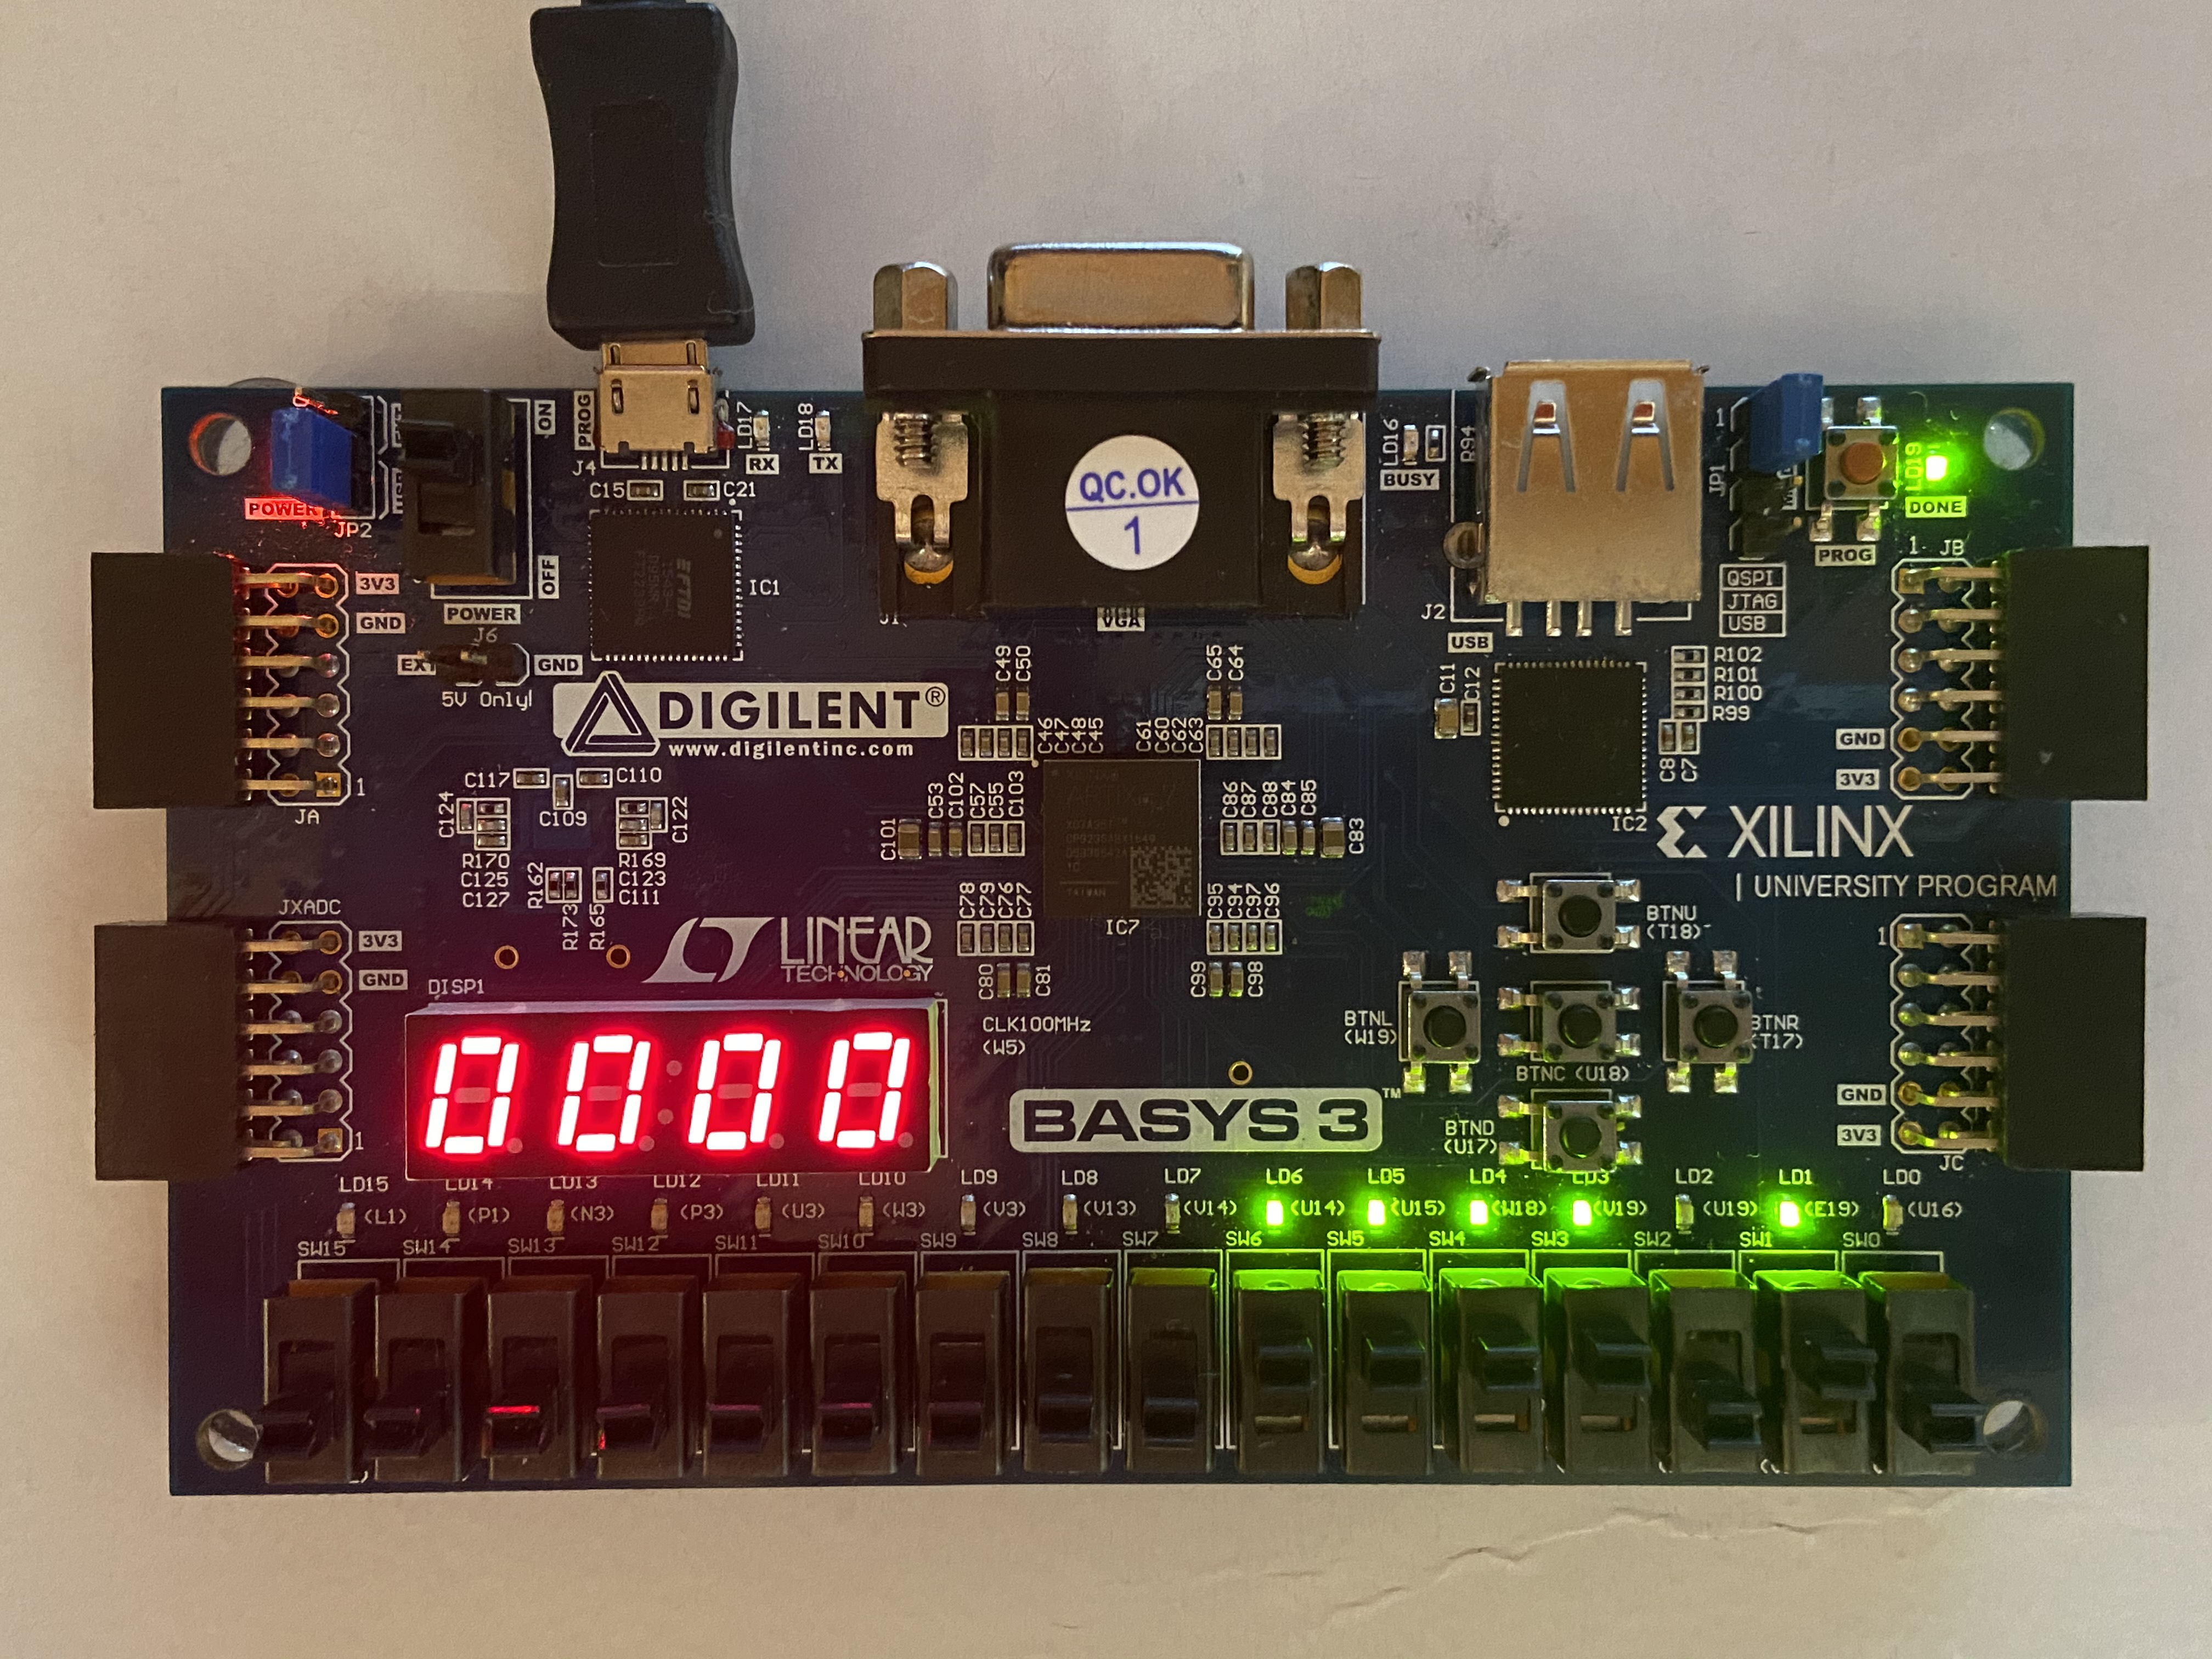
\includegraphics[angle=0, width=1.0\textwidth]{IMG_6747.jpg}
	\caption{Testing Step 2}
	\label{fig:sim_with_table}
\end{figure}
\clearpage

\begin{figure}[ht]\centering
	\includegraphics[angle=0, width=1.0\textwidth]{IMG_6748.jpg}
	\caption{Testing Step 3}
	\label{fig:sim_with_table}
\end{figure}
\clearpage

\begin{figure}[ht]\centering
	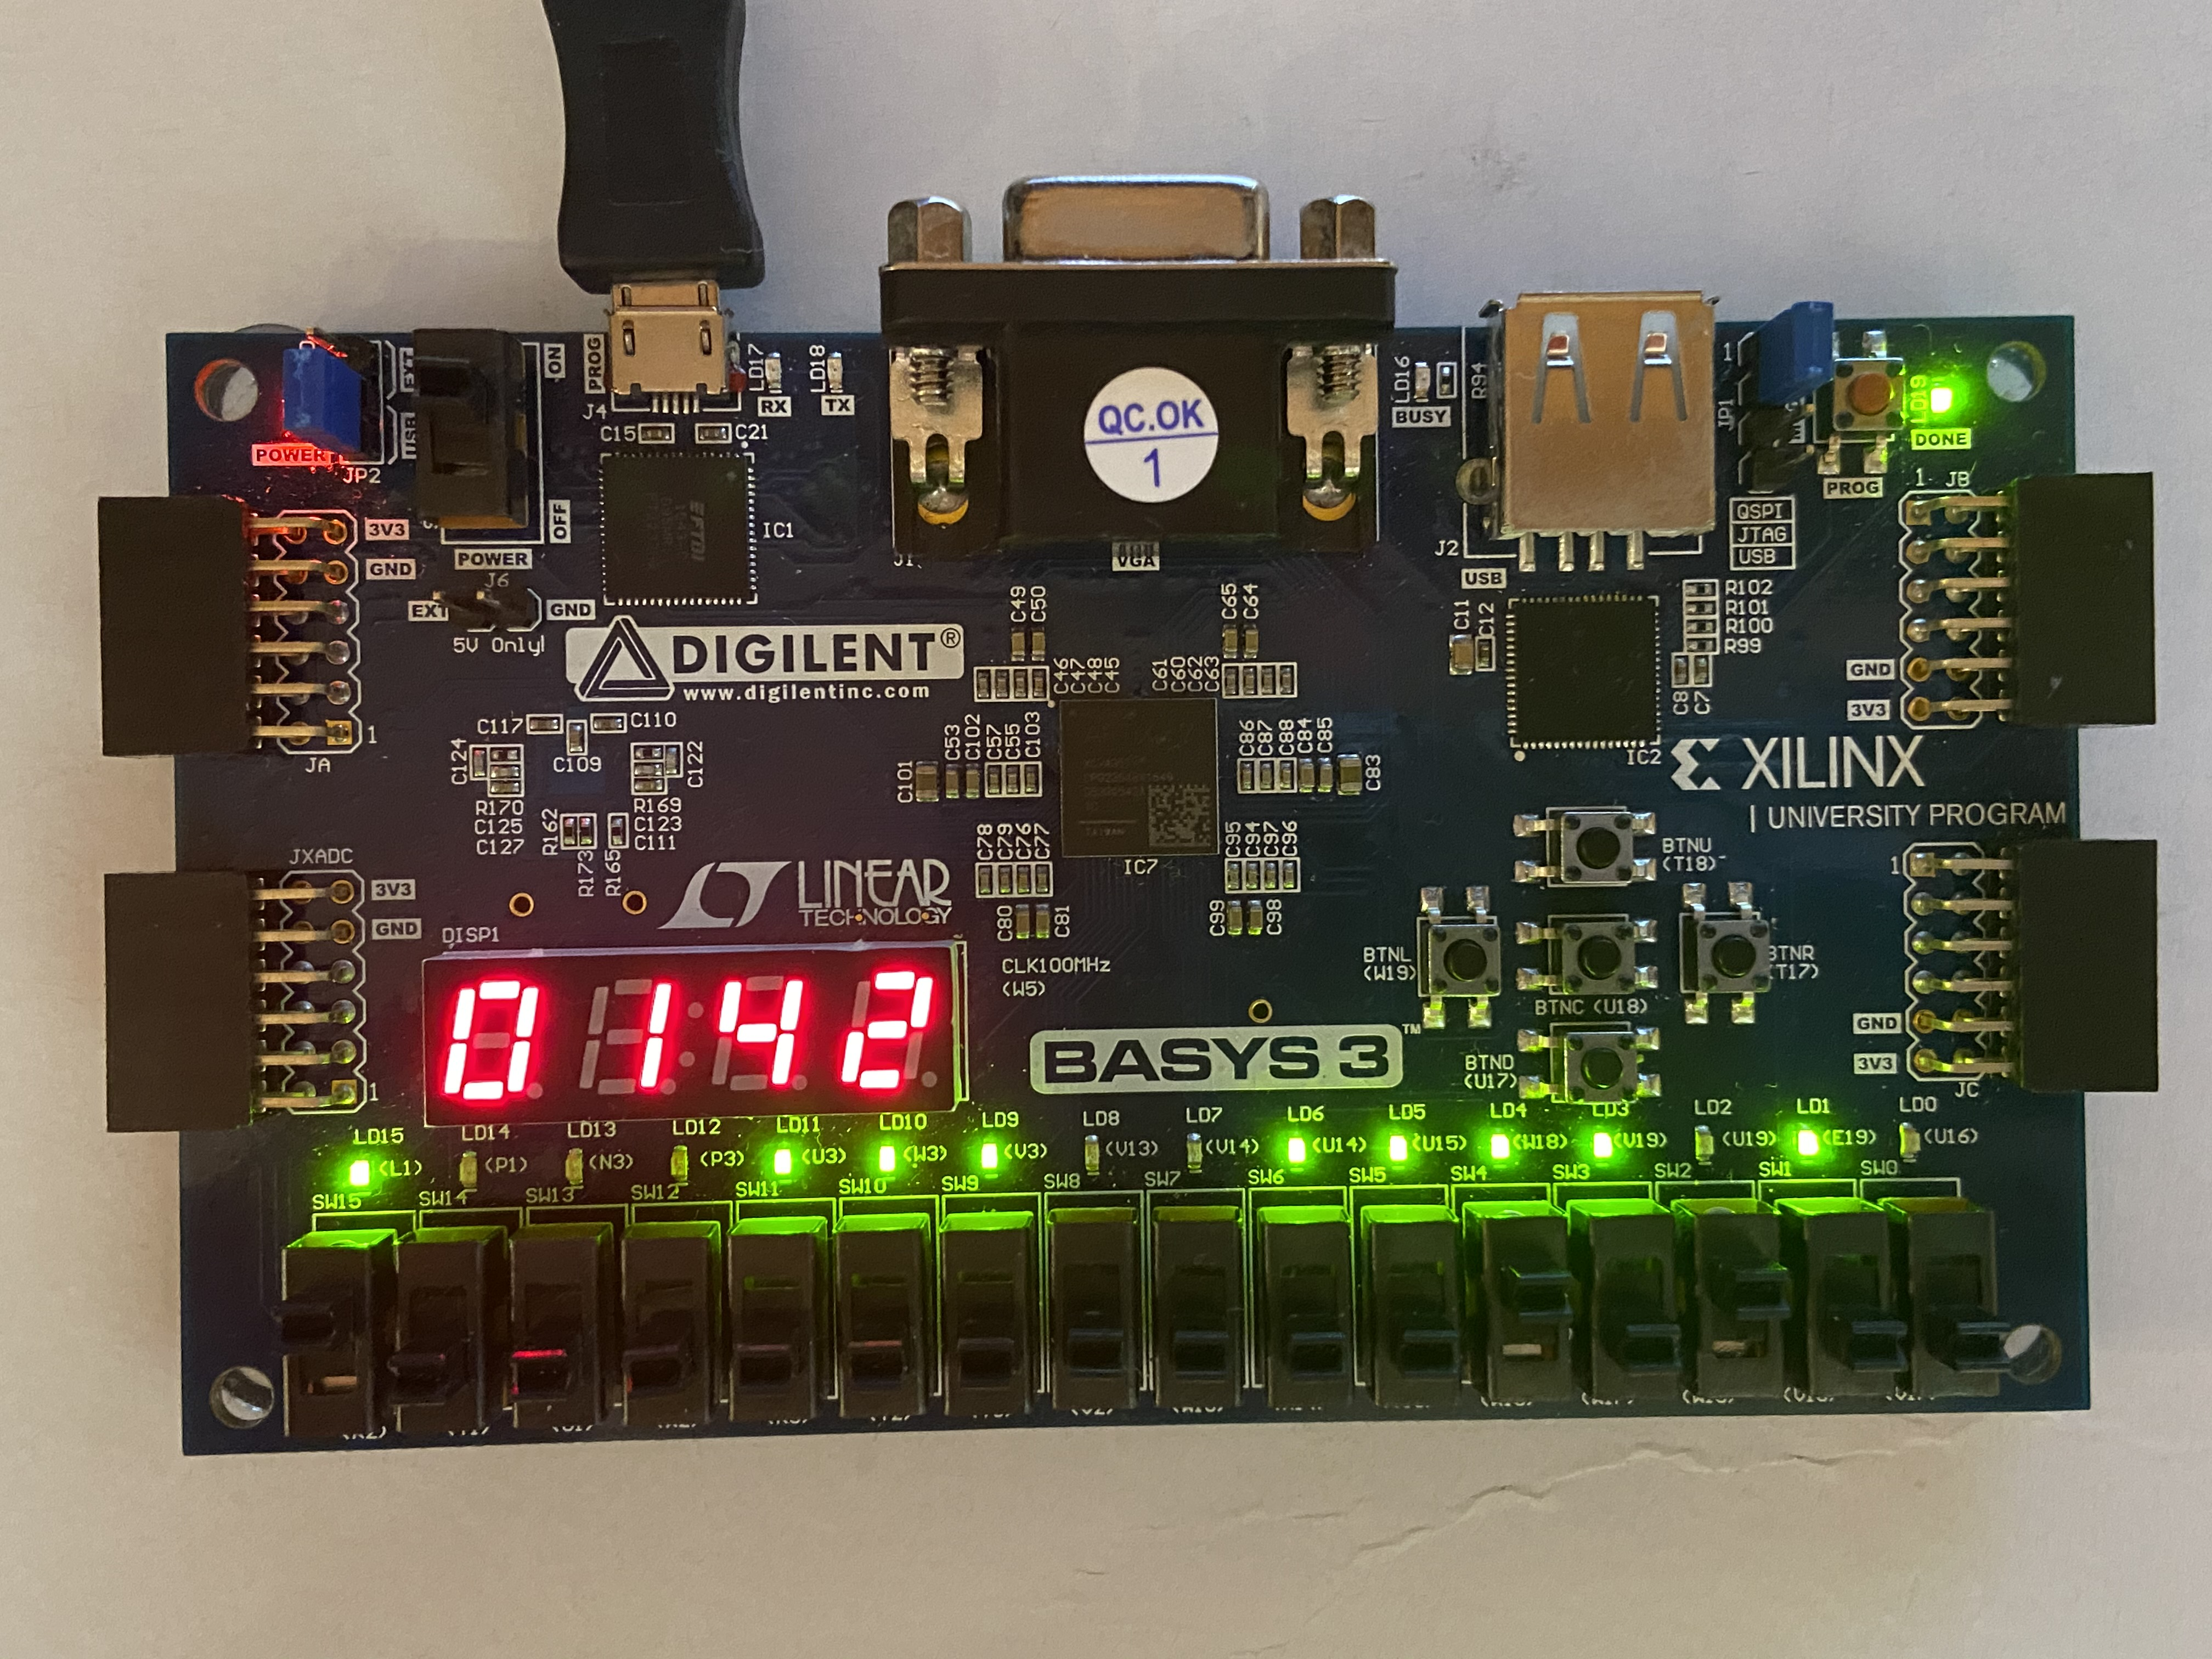
\includegraphics[angle=0, width=1.0\textwidth]{IMG_6749.jpg}
	\caption{Testing Step 4}
	\label{fig:sim_with_table}
\end{figure}
\clearpage

\begin{figure}[ht]\centering
	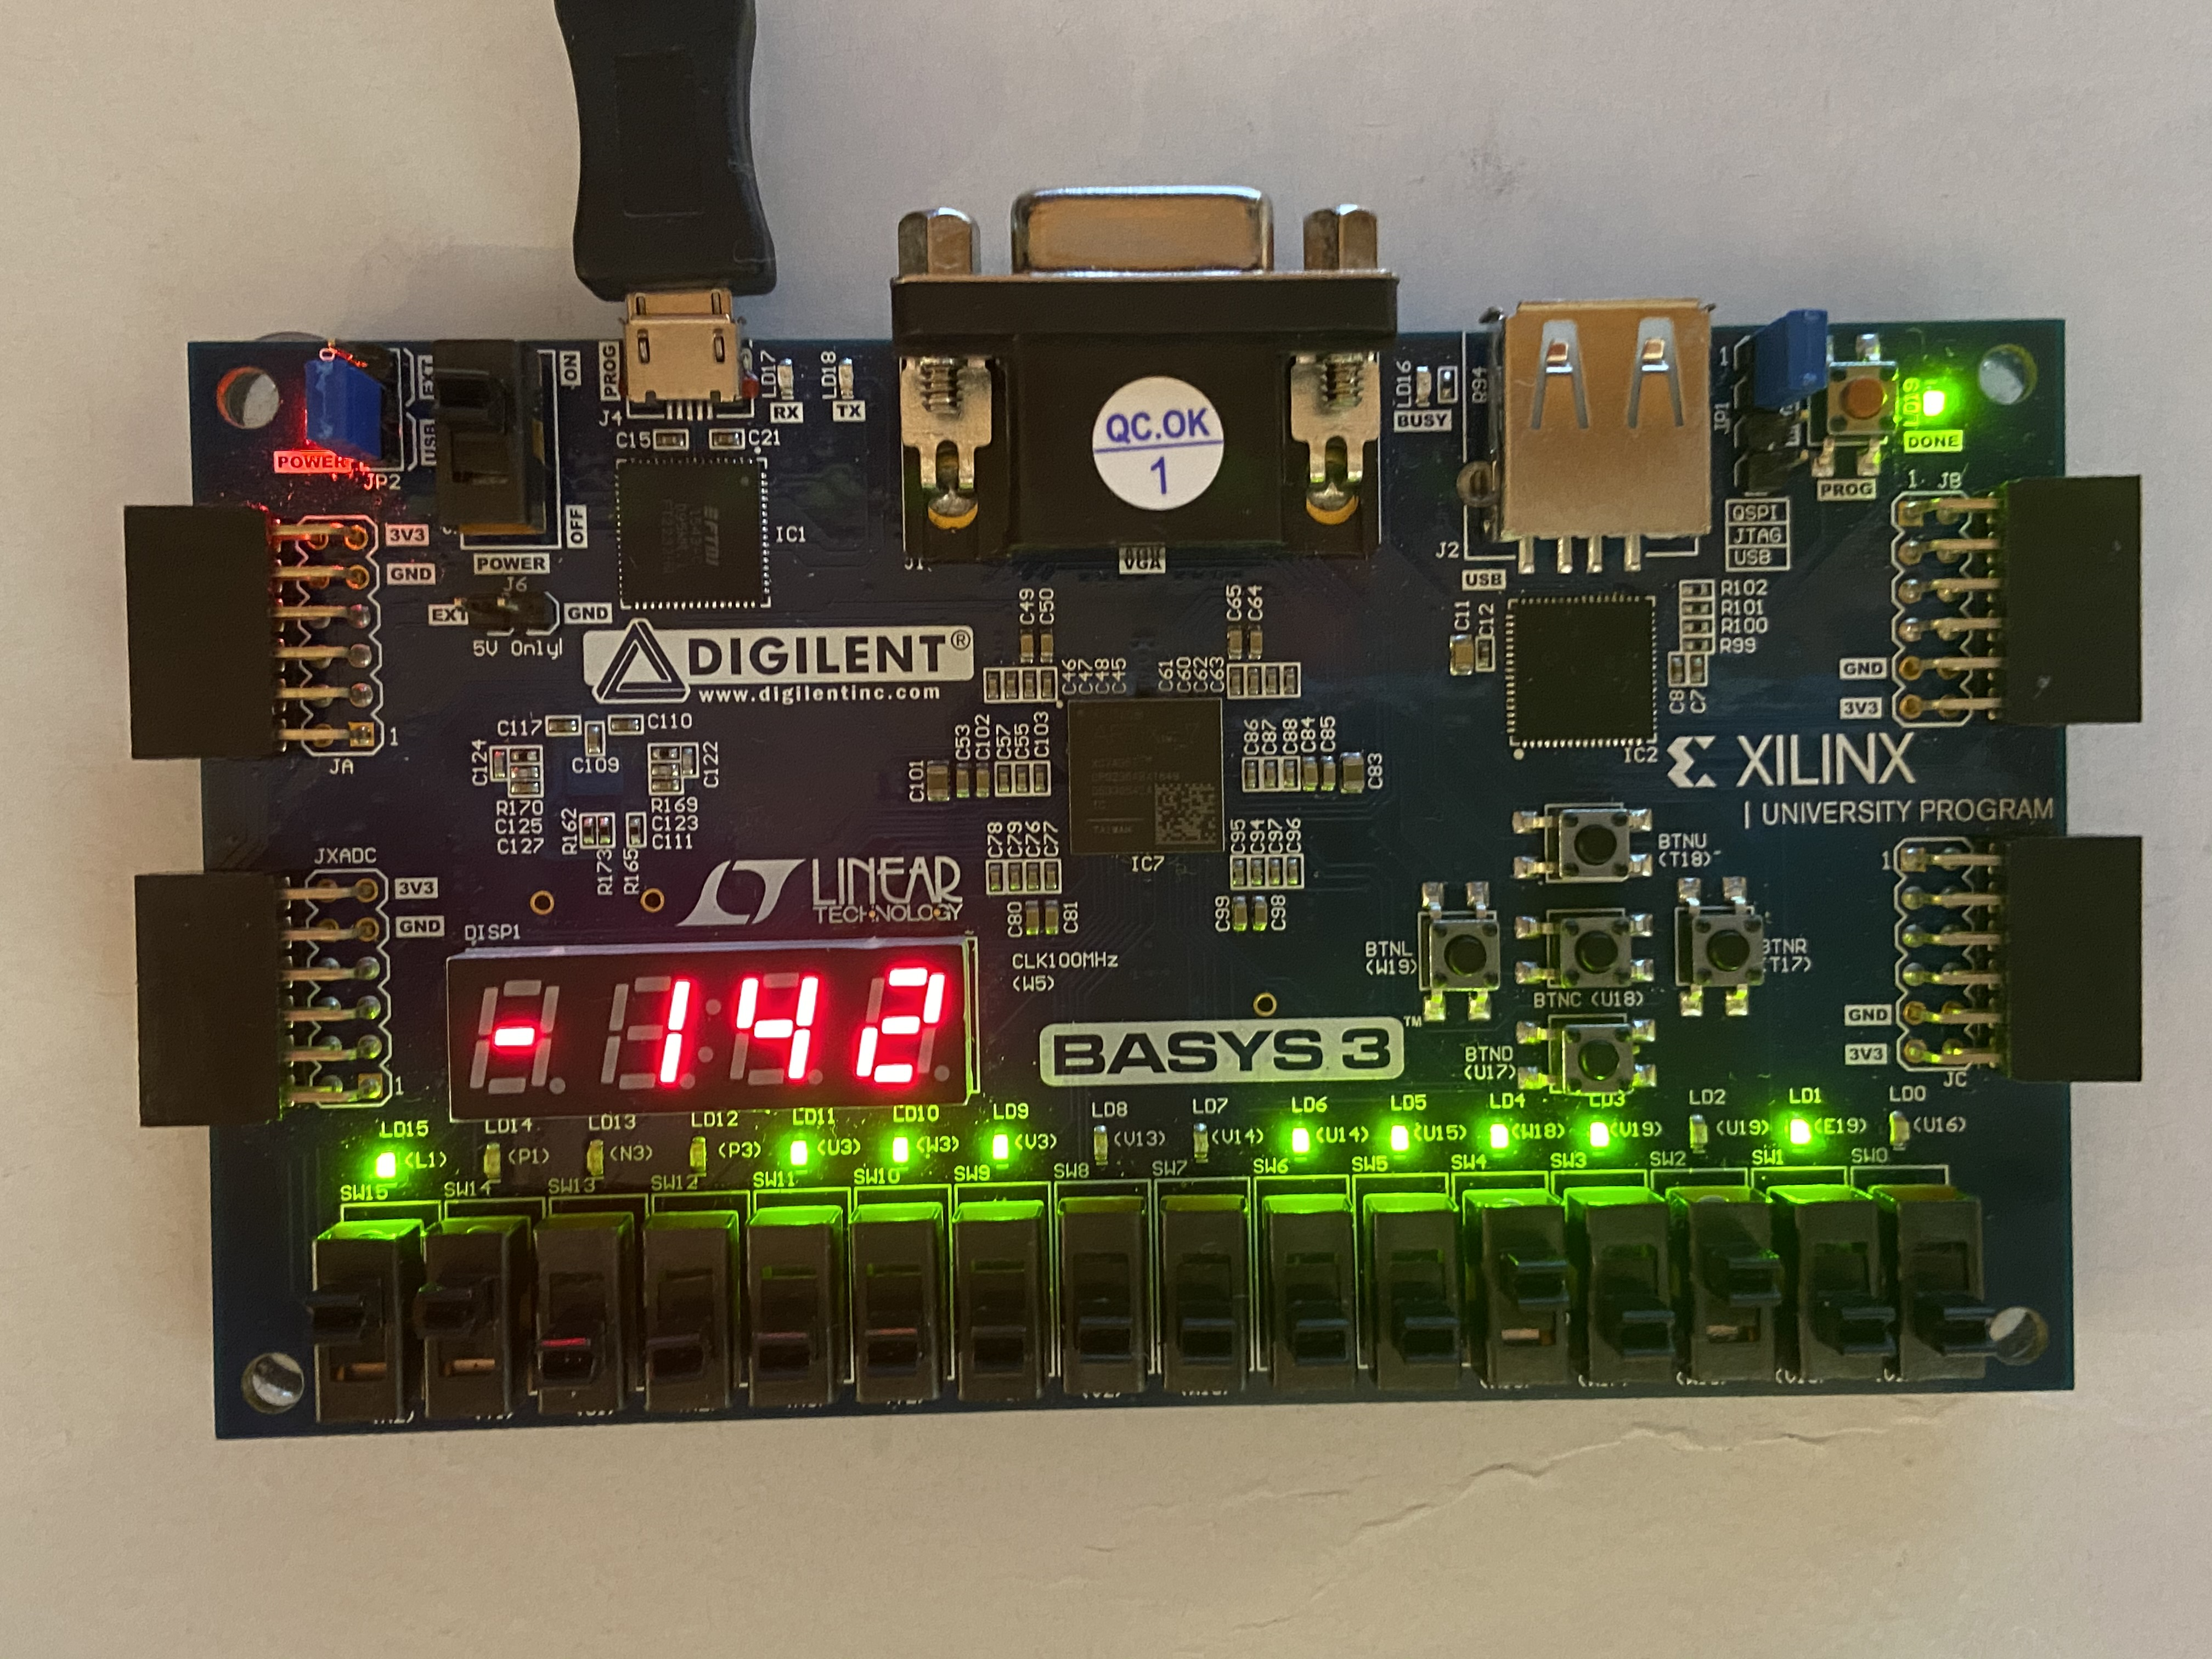
\includegraphics[angle=0, width=1.0\textwidth]{IMG_6750.jpg}
	\caption{Testing Step 5}
	\label{fig:sim_with_table}
\end{figure}
\clearpage

\section*{Code}

Code for source files for Counter, 7-Seg Driver, and Top-Level Calculator and the test bench files for the Counter and Driver.

\begin{lstlisting}[style=Verilog,caption=Counter Code,label=code:ex ]

`timescale 1ns / 1ps
//Megan Gordon, ELC 2137, 2020-04-09

module counter #(parameter N=1)
(input clk, rst, en,
output [N-1:0] count,
output tick
);

//internal signals
reg [N-1:0] Q_reg, Q_next;

//register (state memory)
always @(posedge clk, posedge rst)
begin
if (rst)
Q_reg <= 0;
else
Q_reg <= Q_next;
end

//next-state logic
always @*
begin
if (en)
Q_next = Q_reg + 1;
else
Q_next = Q_reg; //no change
end

//output logic
assign count = Q_reg;
assign tick = (Q_reg=={N{1'b1}}) ? 1'b1 : 1'b0;

endmodule //counter

\end{lstlisting}
\clearpage

\begin{lstlisting}[style=Verilog,caption=7-Seg Driver Code,label=code:ex ]

`timescale 1ns / 1ps
//Megan Gordon, ELC 2137, 2020-04-09

module sseg4_TDM(input [15:0] data,
input hex_dec,sign,
output reg [6:0] seg,
output reg dp,
output reg [3:0] an,
input rst, clk);

wire [1:0] digit_sel;
wire tick1;

counter #(.N(18))timer(.clk(clk), .rst(rst), .en(1'd1), .tick(tick1));


counter #(.N(2))counter2(.clk(tick1), .rst(rst), .en(1'd1), .count(digit_sel));

wire [15:0] bcd11out;
bcd11 sseg4_bcd11(.B(data[10:0]), .Boutfinal(bcd11out));

wire [15:0] mux2_1_out;
mux2 #(.N(16))sseg4_mux2_1(.in0(data[15:0]), .in1(bcd11out), .sel(hex_dec), .out(mux2_1_out));

wire [3:0] mux4_out;
mux4 sseg4_mux4(.in0(mux2_1_out[3:0]), .in1(mux2_1_out[7:4]),.in2(mux2_1_out[11:8]), .in3(mux2_1_out[15:12]), .sel(digit_sel), .out(mux4_out));

wire [6:0]sseg_decoder_out;
sseg_decoder sseg4_decode(.num(mux4_out), .sseg(sseg_decoder_out));

wire [3:0] decoder_out;
an_decode an_decode_sseg4(.in(digit_sel), .out(decoder_out));

wire mux22_in; 
assign mux22_in = ~decoder_out[3] & sign; 
mux2 #(.N(7)) sseg4_mux2_2(.in0(sseg_decoder_out), .in1(7'b0111111), .sel(mux22_in), .out(seg));

assign dp = 1;
assign an = decoder_out;

endmodule

\end{lstlisting}
\clearpage

\begin{lstlisting}[style=Verilog,caption=Top-Level Calculator Code,label=code:ex ]

`timescale 1ns / 1ps
//Megan Gordon, ELC 2137, 2020-04-09

module calc_lab10(
input btnU,
input btnD,
input [15:0]sw,
input clk,
input btnC,
output [15:0]led,
output [6:0] seg,
output dp,
output [3:0] an);

sseg4_TDM disp_unit(.data({8'b00000000, led[15:8]}), 
.hex_dec(sw[15]), .sign(sw[14]), .clk(clk), .rst(btnC), 
.seg(seg), .dp(dp), .an(an));

top_lab9 calc_unit(.btnC(btnC), .btnD(btnD), .btnU(btnU), .clk(clk),
.sw(sw), .led(led));

endmodule

\end{lstlisting}
\clearpage

\begin{lstlisting}[style=Verilog,caption=Counter Test Bench Code,label=code:ex ]

`timescale 1ns / 1ps
//Megan Gordon, ELC 2137, 2020-04-09

module counter_test();

reg clk;
wire [3:0] count;
wire clkA;
wire clkB;
wire clkC;
reg en, rst;

assign clkA = count[0];
assign clkB = count[1];
assign clkC = count[2];

counter #(.N(4)) r(.clk(clk), 
.en(en), .rst(rst), .count(count));

always begin 
clk = ~clk; #5;
end //clock constantly runs

initial begin
clk=0; rst=0; en=0; #5;
rst=1; #5; //reset
rst=0; en=1; #5;
en=0; #5; en=1; #5
en=0; #5; en=1; #5
en=0; #5; en=1; #5
en=0; #5; en=1; #5
en=0; #5; en=1; #5
en=0; #5; en=1; #5
en=0; #5; en=1; #5
en=0; #5; en=1; #5
en=0; #5; en=1; #5
en=0; #5;
$finish;
end

endmodule

\end{lstlisting}
\clearpage

\begin{lstlisting}[style=Verilog,caption=7-Seg Driver Test Bench Code,label=code:ex ]

`timescale 1ns / 1ps
//Megan Gordon, ELC 2137, 2020-04-09

module sseg4_TDM_test();


reg [15:0] data;
reg hex_dec,sign;
wire [6:0] seg;
wire dp;
wire [3:0] an;
reg rst, clk;


sseg4_TDM testTDM(.clk(clk), .rst(rst), .data(data), .seg(seg), .dp(dp), .an(an),
.hex_dec(hex_dec), .sign(sign));

always begin 
clk = ~clk; #10;
end //clock constantly runs

initial begin
clk=0; rst=1;
hex_dec=0; sign=0;
data=16'b0001011001110011;
#2621440;
rst=0; #26214400;
hex_dec=1; #26214400;
sign=1; 
end

endmodule

\end{lstlisting}

\end{document}
